\documentclass[conference]{IEEEtran}
\IEEEoverridecommandlockouts
\usepackage{standalone}
\usepackage{tikz} % O los paquetes que use tu figura
\usepackage{tikz-3dplot}
\usepackage{cite}
\usepackage{amsmath,amssymb,amsfonts}
\usepackage{algorithmic}
\usepackage{graphicx}
\usepackage{textcomp}
\usepackage{xcolor}
\usepackage{float}
\usepackage{booktabs}
\usepackage{url}
% -------Ajuste fino de espaçamento de figuras (IEEE-safe)-----------
%\setlength{\textfloatsep}{8pt plus 2pt minus 2pt}
%\setlength{\floatsep}{6pt plus 2pt minus 2pt}
%\setlength{\intextsep}{6pt plus 2pt minus 2pt}
%--------------------------------------------------------------------
\DeclareUnicodeCharacter{2060}{}

\def\BibTeX{{\rm B\kern-.05em{\sc i\kern-.025em b}\kern-.08em
    T\kern-.1667em\lower.7ex\hbox{E}\kern-.125emX}}

\begin{document}

\title{Pseudo-Brewster Angle–Guided Bistatic SAR Optimization for Subsurface Sensing}

\author{
\IEEEauthorblockN{
David Atencia Mondagón\IEEEauthorrefmark{1}\IEEEauthorrefmark{4},
Eder Carlos Fernandes\IEEEauthorrefmark{1}\IEEEauthorrefmark{5},
Everton Gomede\IEEEauthorrefmark{2}\IEEEauthorrefmark{6},\\
João Roberto Moreira Neto\IEEEauthorrefmark{3}\IEEEauthorrefmark{7},
Hugo Enrique Hernandez Figueroa\IEEEauthorrefmark{1}\IEEEauthorrefmark{8}
}

\vspace{2pt}
\rule{0.0\linewidth}{0.4pt}
\vspace{4pt}

\IEEEauthorblockA{\IEEEauthorrefmark{1}State University of Campinas (UNICAMP), Campinas/SP 13083-852, Brazil}
\IEEEauthorblockA{\IEEEauthorrefmark{2}University of British Columbia (UBC), Vancouver/BC V6T 1Z4, Canada}
\IEEEauthorblockA{\IEEEauthorrefmark{3}Radaz S.A., São José dos Campos/SP 02047-901, Brazil}

\vspace{4pt}
\IEEEauthorblockA{
\IEEEauthorrefmark{4}david.mondagon@embraer.com.br,
\IEEEauthorrefmark{5}e208418@dac.unicamp.br,
\IEEEauthorrefmark{6}everton.gomede@ubc.ca, \\
\IEEEauthorrefmark{7}tech@radaz.com.br,
\IEEEauthorrefmark{8}hugo@unicamp.br
}
}

\maketitle

\begin{abstract}
This paper presents a physics-guided optimization framework for bistatic synthetic aperture radar (SAR) data acquisition aimed at subsurface sensing applications. The proposed approach integrates pseudo-Brewster-angle-based flight planning with receiver positioning to improve electromagnetic transmission through the air-ground interface in lossy dielectric media. A QGIS-based flight-planning tool was developed to generate bistatic drone trajectories conditioned on pseudo-Brewster-angle constraints and integrated with the RD350 Explorer drone-borne SAR system. Receiver placement is formulated as a multi-start optimization problem with physically motivated initialization strategies derived from electromagnetic transmission theory. Simulations conducted at 400 MHz indicate that pseudo-Brewster-guided bistatic geometries achieve the highest average received power (-70.11 dBm), compared with the perpendicular (-72.99 dBm) and opposite (-72.30 dBm) configurations. All reported values are averages across multiple target configurations and initialization seeds. The results indicate that explicitly incorporating electromagnetic transmission physics into bistatic SAR geometry design can yield measurable coupling gains in simulations. Experimental and reconstruction-level validation of the resulting data quality improvements is ongoing.
\end{abstract}

\begin{IEEEkeywords}
Bistatic SAR, Pseudo-Brewster Angle, Receiver Optimization, Flight Planning, Subsurface Sensing
\end{IEEEkeywords}

\section{Introduction}

Subsurface investigation at depths of hundreds of meters remains a significant challenge for conventional radar systems \cite{daniels_gpr}. Ground-penetrating radar (GPR) techniques are typically limited to penetration depths of only a few tens of meters due to electromagnetic attenuation, whereas emerging applications such as mineral exploration, archaeological surveys, and groundwater detection demand deeper, more reliable sensing capabilities \cite{Soil}.

Bistatic radar systems, where transmitter and receiver are spatially separated, offer significant potential for enhanced penetration capabilities \cite{cherniakov_bistatic}. However, the effectiveness of these systems critically depends on the electromagnetic coupling efficiency at the air-ground interface, which is highly sensitive to the angle of incidence at lossy dielectric interfaces.
The pseudo-Brewster angle maximizes electromagnetic transmission in lossy media \cite{mcmichael_brewster} and, when incorporated into system design, provides a physics-based criterion for improving subsurface sensing configurations.

The proposed system integrates: (1) pseudo-Brewster-angle-based flight planning, (2) bistatic receiver optimization, and (3) an integrated drone-borne SAR platform. This work contributes an optimization workflow that integrates electromagnetic theory, mission planning, and SAR acquisition to support improved acquisition conditions for subsurface tomography processing.

Prior studies have typically addressed bistatic SAR geometry design, electromagnetic interface modeling, and UAV mission planning as decoupled problems. This work proposes an integrated, operationally viable framework that unifies electromagnetic transmission theory, bistatic geometry optimization, and mission planning for drone-borne SAR systems. The main contribution of this paper lies in the explicit incorporation of pseudo-Brewster-angle physics into both flight-trajectory design and receiver-placement optimization, enabling measurable improvements in electromagnetic coupling at the air-ground interface and supporting improved acquisition conditions for subsequent tomographic processing.

\section{Related Work and Theoretical Foundation}

This section reviews the electromagnetic principles underlying pseudo-Brewster-angle optimization in bistatic SAR systems and summarizes related work that motivates its use in subsurface sensing.

\subsection{Pseudo-Brewster Angle in Lossy Media}

The fundamental theory governing maximum transmission at interfaces for media with complex permittivity has been established for ground-penetrating radar applications. While the classical Brewster angle does not exist in lossy soils, a pseudo-Brewster angle that depends on complex permittivity (real and imaginary parts) provides practical optimization guidance \cite{mcmichael_brewster}.

For lossy media, the pseudo-Brewster angle minimizes reflection and maximizes transmission efficiency \cite{mcmichael_brewster}. This angle varies primarily with soil moisture and frequency, making it an important parameter for mission planning in subsurface sensing applications.

\subsection{Bistatic Radar for Subsurface Sensing}

Recent research has advanced the use of drone-transported SAR systems operating in multiple bands (P, L, C) for surface and shallow subsurface sensing applications. Studies have applied these systems for agricultural soil moisture mapping and subsurface anomaly detection in controlled experiments using linear and helical flight trajectories \cite{ore_soil_moisture}.

The bistatic radar equation for subsurface targets must account for electromagnetic wave transmission through multiple media, including refraction and attenuation at the air–ground interface, as expressed in Eq.~\ref{eq:bistatic_radar}:

\begin{equation}
P_r = \frac{P_t G_t G_r \sigma T_{tx} T_{rx} \lambda^2}{(4\pi)^3 R_1^2 R_2^2 R_3^2 R_4^2}
\label{eq:bistatic_radar}
\end{equation}

where $P_t$ denotes the transmitted power, $G_t$ and $G_r$ are the transmitter and receiver antenna gains, respectively, $\sigma$ represents the radar cross section of the subsurface target, $T_{tx}$ and $T_{rx}$ are the power transmittance coefficients at the air–ground interface for the transmit and receive paths, $\lambda$ is the operating wavelength, and $R_1, R_2, R_3, R_4$ denote the individual propagation path segments illustrated in Figure~\ref{fig:bistatic_geometry}.

\begin{figure}[ht]
\centering
\scalebox{0.6}{% Figura 1: Geometría del sistema bistático
\documentclass[border=5pt]{standalone}
\usepackage{tikz}
\usepackage{tikz-3dplot}
\usetikzlibrary{arrows.meta, decorations.pathreplacing, calc} % <-- ADICIONAR calc

\begin{document}
\tdplotsetmaincoords{70}{110}

\begin{tikzpicture}[tdplot_main_coords, scale=0.8]

% Definir puntos
\coordinate (Tx) at (2, 4, 3);
\coordinate (Rx) at (-3, -2, 3);
\coordinate (Target1) at (0, 0, -2);
\coordinate (Target2) at (1, 1, -2);
\coordinate (Surface1) at (0.8, 1.6, 0);
\coordinate (Surface2) at (-0.6, -0.4, 0);

% Plano del suelo
\fill[gray!20, opacity=0.5] (-4,-4,0) -- (4,-4,0) -- (4,4,0) -- (-4,4,0) -- cycle;
\draw[gray] (-4,-4,0) -- (4,-4,0) -- (4,4,0) -- (-4,4,0) -- cycle;

% Subsuelo
\fill[brown!30, opacity=0.3] (-4,-4,-3) -- (4,-4,-3) -- (4,4,-3) -- (-4,4,-3) -- 
                              (-4,-4,0) -- (4,-4,0) -- (4,4,0) -- (-4,4,0) -- cycle;

% Transmisor
\draw[blue, thick] (Tx) circle (0.15);
\fill[blue] (Tx) circle (0.1);
\node[above, blue] at (Tx) {Transmitter};

% Receptor
\draw[red, thick] (Rx) circle (0.15);
\fill[red] (Rx) circle (0.1);
\node[above, red] at (Rx) {Receiver};

% Targets
\foreach \target in {Target1, Target2} {
    \draw[black, thick] (\target) circle (0.1);
    \fill[black] (\target) circle (0.08);
}
\node[below] at (Target1) {Target 1};
\node[below] at (Target2) {Target 2};

% Trayectorias de rayos
% Tx → Surface1 → Target1
\draw[blue, thick, ->] (Tx) -- (Surface1);
\draw[blue, thick, dashed, ->] (Surface1) -- (Target1);

% Target1 → Surface2 → Rx
\draw[red, thick, dashed, ->] (Target1) -- (Surface2);
\draw[red, thick, ->] (Surface2) -- (Rx);

% Etiquetas de distancias
\node[midway, above] at ($(Tx)!0.5!(Surface1)$) {$R_1$};
\node[midway, right] at ($(Surface1)!0.5!(Target1)$) {$R_2$};
\node[midway, left] at ($(Target1)!0.5!(Surface2)$) {$R_3$};
\node[midway, below] at ($(Surface2)!0.5!(Rx)$) {$R_4$};

% Puntos de intersección
\fill[green] (Surface1) circle (0.05);
\fill[green] (Surface2) circle (0.05);

% Ejes de coordenadas
\draw[->] (0,0,0) -- (2,0,0) node[right] {$X$};
\draw[->] (0,0,0) -- (0,2,0) node[above] {$Y$};
\draw[->] (0,0,0) -- (0,0,2) node[above] {$Z$};

% Etiquetas de medios
\node[right] at (3, 3, 1.5) {Air ($n_1 = 1$)};
\node[right] at (3, 3, -1.5) {Ground ($n_2 > 1$)};

\end{tikzpicture}
\end{document}}
% \includegraphics[width=0.48\textwidth]{bistatic_geometry.png}
\caption{Bistatic radar geometry for subsurface target detection showing electromagnetic wave paths through the air-ground interface. The system comprises a transmitter (Tx), a receiver (Rx), subsurface targets, and the four path segments $R_1$, $R_2$, $R_3$, and $R_4$, which represent the complete bistatic propagation path.}
\label{fig:bistatic_geometry}
\end{figure}

The power transmittances satisfy energy conservation at the interface and are calculated from the Fresnel transmission coefficient, as shown in Eq.~\ref{eq:power_transmittance}:

\begin{equation}
T = \frac{n_2 \cos \theta_2}{n_1 \cos \theta_1} |t_{TM}|^2
\label{eq:power_transmittance}
\end{equation}

where $n_1$ and $n_2$ are the refractive indices of the incident and transmitted media, $\theta_1$ and $\theta_2$ are the corresponding propagation angles, and $t_{\mathrm{TM}}$ is the Fresnel transmission coefficient for TM polarization.

\section{System Architecture and Methodology}

The integrated system employs a quantitative experimental approach, comprising four main components that form a comprehensive data acquisition and processing pipeline.

\subsection{Flight Planning Application with QGIS Integration}

A QGIS Python plugin computes pseudo-Brewster angles for lossy media from soil-permittivity inputs (Table~\ref{tab:soil_permittivity}) and generates flight plans for bistatic drone configurations.

\begin{table}[hbt]
\centering
\caption{Soil Complex Permittivity vs. Moisture Content}
\label{tab:soil_permittivity}
\begin{tabular}{rc}
\toprule
\textbf{Soil Moisture (\%)} & \textbf{Complex Permittivity} \\
\midrule
20 & $12.1643 - 4.6751i$ \\
25 & $15.536 - 5.4890i$ \\
30 & $19.2249 - 6.2653i$ \\
35 & $23.2166 - 7.0153i$ \\
40 & $27.4989 - 7.7397i$ \\
45 & $32.0616 - 8.4485i$ \\
\bottomrule
\end{tabular}
\end{table}

Soil characterization and pseudo-Brewster-angle analysis were performed using electromagnetic simulations in Python, with fixed permittivity values obtained from FEAGRI (Unicamp). For each moisture condition, one representative simulation was conducted to establish a physics-based reference for flight planning rather than to support statistical inference.

Three independent tests were executed, corresponding to three distinct radii of the helical trajectory from the top to the base of the volume of interest. For each test, geometric feasibility was strictly conditioned on satisfying the pseudo-Brewster angle. Configurations that failed to meet this condition did not produce a valid illuminated area and were consequently discarded.

These soil-characterization data were used to generate reflectivity curves. For flight-planning analysis, we considered the curves for the driest and wettest soil conditions shown in Fig.~\ref{fig:optimal_range}, which illustrate the relationship between the incidence angle and electromagnetic coupling efficiency.

\begin{figure}[ht]
\centering
\includegraphics[width=0.35\textwidth]{Reflection_Coefficient_Pseudo_Brewster_V2.png}
\caption{Optimal reflectivity range (0.2) for moisture conditions between 20\% and 45\%, used for flight planning optimization in the QGIS plugin.}
\label{fig:optimal_range}
\end{figure}

The plugin automatically generates flight plans for bistatic configurations using two drones positioned with conical spiral trajectories. The drones are positioned 180° apart along a spiral trajectory, with paths constrained by the calculated pseudo-Brewster-angle range.

\subsection{Multi-Band SAR Acquisition System}

The proposed framework uses the RD350 Explorer, a multi-band synthetic aperture radar (SAR) operating in P, L, and C bands and designed for drone-based operation. For the present study, all simulations and optimization experiments were conducted at a carrier frequency of 400 MHz (UHF band), selected to balance subsurface penetration capabilities with practical antenna dimensions and spatial resolution requirements. The system includes microwave sensors, antennas, a GNSS ground station, and integrated software for planning and processing.

The commissioning process verified hardware-software integration and field-flight execution capability. Tomographic acquisition flights follow the flight plans generated by the QGIS plugin to maintain favorable electromagnetic coupling throughout data collection.

\subsection{Bistatic Receiver Optimization}

The receiver positioning optimization is formulated as (Eq.~\ref{eq:optimization_problem}):

\begin{equation}
\max_{\mathbf{r}_r} \sum_{i=1}^{N_t} P_{r,i}(\mathbf{r}_r)
\label{eq:optimization_problem}
\end{equation}

subject to geometric constraints, where $N_t$ is the number of targets and $P_{r,i}$ is the received power from the $i$-th target. The current experiments assume homogeneous target reflectivity ($\sigma_i = \sigma$); weighted variants, such as $\sum w_i P_{r,i}$, and max-min robust formulations are natural extensions for heterogeneous scenes.

Received power was selected as the optimization objective because it directly reflects electromagnetic transmission efficiency at the air-ground interface and is strongly influenced by the pseudo-Brewster angle. Maximizing received power, therefore, provides a physics-based criterion that is independent of specific signal-processing assumptions.

While metrics such as SNR, ambiguity, and coherence loss are crucial for assessing image quality, they depend on additional factors, including bandwidth, processing algorithms, and platform stability. They are therefore most appropriately evaluated at the processing stage. It is worth noting that range and azimuth resolution are fundamentally governed by system bandwidth and synthetic aperture length, respectively, and are not directly improved by power optimization. Instead, higher received power is expected to improve the acquisition-domain SNR margin, which may extend effective detection coverage---the volume fraction of targets above the detectability threshold---and improve localization precision by increasing the peak-to-sidelobe ratio available to reconstruction estimators. The proposed framework, therefore, targets coverage and precision, rather than resolution, as its primary geometry-level outcomes.

Five initialization strategies were implemented: geometric opposition, perpendicular positioning, and Brewster-guided approaches (Eq.~\ref{eq:brewster_position}), with the latter using pseudo-Brewster-angle calculations to define physically informed initial placements.

\begin{equation}
\mathbf{r}_{ref} = \mathbf{c}_t + d_B \begin{bmatrix} \cos(\phi_{opp}) \\ \sin(\phi_{opp}) \end{bmatrix}
\label{eq:brewster_position}
\end{equation}

where $d_B = h_{total}/\tan(\theta_B)$ is the Brewster distance and $\theta_B$ is the pseudo-Brewster angle, as shown in Figure~\ref{fig:optimization_strategies}.

\begin{figure}[ht]
\centering
\scalebox{0.55}{% Figura 2: Estrategias de optimización
\documentclass[border=5pt]{standalone}
\usepackage{tikz}
\usetikzlibrary{arrows.meta, decorations.pathreplacing, patterns}

\begin{document}

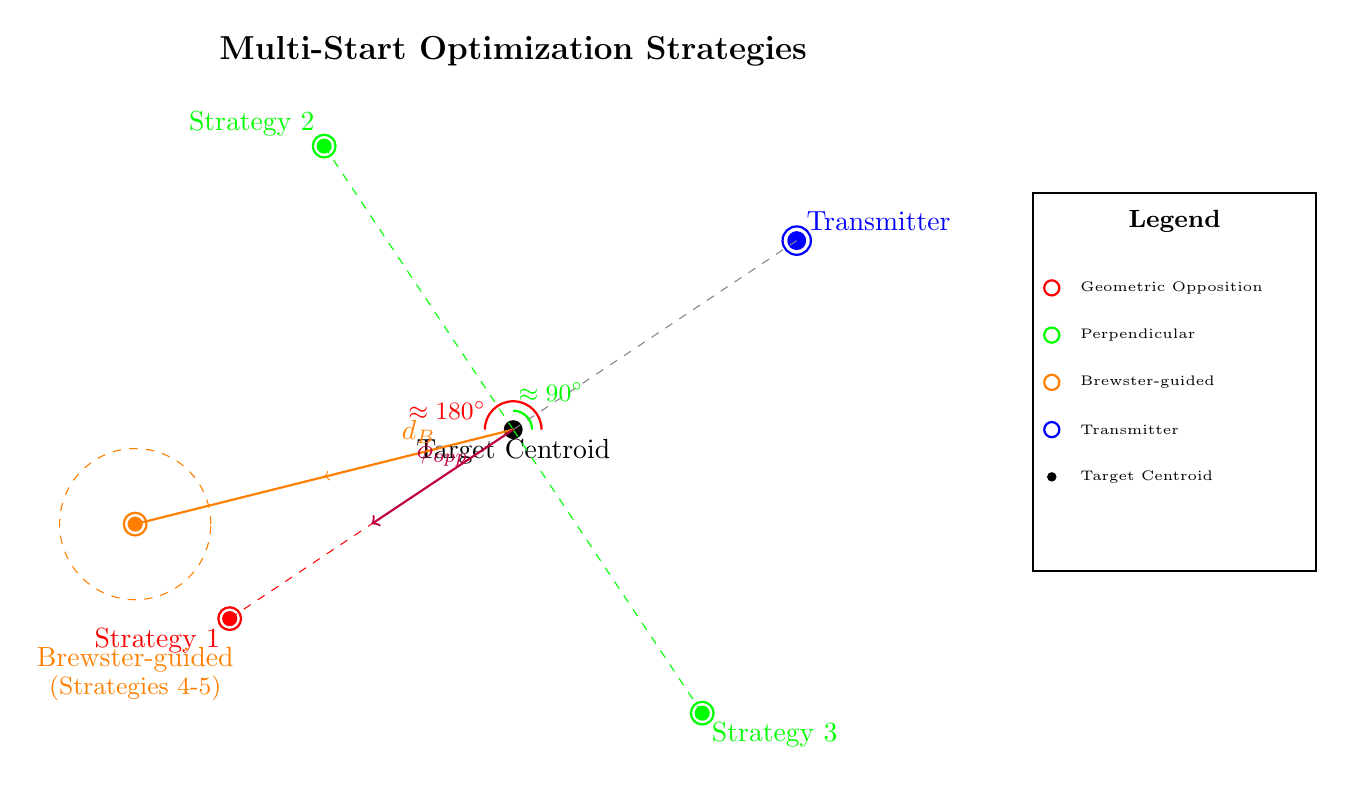
\begin{tikzpicture}[scale=1.2]

% Centro de targets
\coordinate (Center) at (0, 0);
\fill[black] (Center) circle (0.1);
\node[below] at (Center) {Target Centroid};

% Transmisor
\coordinate (Tx) at (3, 2);
\draw[blue, thick] (Tx) circle (0.15);
\fill[blue] (Tx) circle (0.1);
\node[above right, blue] at (Tx) {Transmitter};

% Línea Tx-Center
\draw[gray, dashed] (Tx) -- (Center);

% Estrategia 1: Posición opuesta
\coordinate (Rx1) at (-3, -2);
\draw[red, thick] (Rx1) circle (0.12);
\fill[red] (Rx1) circle (0.08);
\node[below left, red] at (Rx1) {Strategy 1};
\draw[red, dashed] (Center) -- (Rx1);

% Estrategia 2: Perpendicular
\coordinate (Rx2) at (-2, 3);
\draw[green, thick] (Rx2) circle (0.12);
\fill[green] (Rx2) circle (0.08);
\node[above left, green] at (Rx2) {Strategy 2};
\draw[green, dashed] (Center) -- (Rx2);

% Estrategia 3: Perpendicular opuesta
\coordinate (Rx3) at (2, -3);
\draw[green, thick] (Rx3) circle (0.12);
\fill[green] (Rx3) circle (0.08);
\node[below right, green] at (Rx3) {Strategy 3};
\draw[green, dashed] (Center) -- (Rx3);

% Estrategia 4-5: Brewster-guided (con zona de aleatoriedad)
\coordinate (RxBrewster) at (-4, -1);
\draw[orange, thick] (RxBrewster) circle (0.12);
\fill[orange] (RxBrewster) circle (0.08);

% Zona de aleatoriedad alrededor del punto Brewster
\draw[orange, dashed] (RxBrewster) circle (0.8);
\node[below, orange] at (-4, -2.2) {Brewster-guided};
\node[below, orange, font=\small] at (-4, -2.5) {(Strategies 4-5)};

% Ángulo de Brewster ilustrativo
\draw[orange, thick] (Center) -- (RxBrewster);
\draw[orange, ->] (Center) -- (-2, -0.5) node[midway, above] {$d_B$};

% Azimut opuesto
\draw[purple, thick, ->] (Center) -- (-1.5, -1) node[midway, above] {$\phi_{opp}$};

% Ángulo bistático para Strategy 1
\draw[red, thick] (Center) ++(0.3, 0) arc (0:180:0.3);
\node[red, font=\small] at (-0.7, 0.2) {$\approx 180^\circ$};

% Ángulos bistáticos para perpendiculares
\draw[green, thick] (Center) ++(0.2, 0) arc (0:90:0.2);
\node[green, font=\small] at (0.4, 0.4) {$\approx 90^\circ$};

% Etiquetas adicionales
\node[font=\large\bfseries] at (0, 4) {Multi-Start Optimization Strategies};

% Leyenda
\begin{scope}[shift={(5.5, 1)}]
    \draw[thick] (0, 1.5) rectangle (3, -2.5);
    \node[font=\small\bfseries] at (1.5, 1.2) {Legend};
    
    \draw[red, thick] (0.2, 0.5) circle (0.08);
    \node[font=\tiny, right] at (0.4, 0.5) {Geometric Opposition};
    
    \draw[green, thick] (0.2, 0) circle (0.08);
    \node[font=\tiny, right] at (0.4, 0) {Perpendicular};
    
    \draw[orange, thick] (0.2, -0.5) circle (0.08);
    \node[font=\tiny, right] at (0.4, -0.5) {Brewster-guided};
    
    \draw[blue, thick] (0.2, -1) circle (0.08);
    \node[font=\tiny, right] at (0.4, -1) {Transmitter};
    
    \fill[black] (0.2, -1.5) circle (0.05);
    \node[font=\tiny, right] at (0.4, -1.5) {Target Centroid};
\end{scope}

\end{tikzpicture}
\end{document}}
% \includegraphics[width=0.48\textwidth]{optimization_strategies.png}
\caption{Multi-start optimization strategies for bistatic receiver positioning. Strategy 1 (red) maximizes bistatic angle through geometric opposition. Strategies 2-3 (green) provide perpendicular positioning. Strategies 4-5 (orange) use pseudo-Brewster angle-guided positioning.}
\label{fig:optimization_strategies}
\end{figure}

\subsection{Enhanced Data Quality for Tomographic Processing}

The improved signal conditions achieved through pseudo-Brewster-angle optimization are expected to support more effective tomographic processing. Raw data from the optimized acquisition can be processed using standard time-domain backprojection algorithms to synthesize 3D images of the soil volume from spiral trajectories. The processing includes absolute radiometric calibration performed with corner reflectors.

The received-power gains obtained from electromagnetic optimization create favorable acquisition-domain SNR margins ($\mathrm{SNR} \propto P_r$), which are expected to support improved reconstruction quality; however, gains in penetration depth and tomographic fidelity require controlled inversion experiments for direct confirmation.

\section{Results and Analysis}

This section presents a quantitative evaluation of the proposed pseudo-Brewster-guided bistatic SAR optimization framework. The analysis evaluates the effectiveness of the flight-planning and receiver-positioning strategies by measuring received power at the bistatic receiver, which serves as an indicator of electromagnetic transmission efficiency at the air-ground interface. Simulation results obtained at a carrier frequency of 400~MHz are used to compare Brewster-guided positioning with perpendicular and geometric opposition configurations, highlighting the electromagnetic advantages of the proposed approach.

\subsection{Flight Planning Validation}

The QGIS plugin successfully computed pseudo-Brewster-angle ranges for different moisture conditions and generated viable flight plans. Integration with the RD350 drone control software was established, enabling mission execution based on the generated plans.

The optimization framework consistently identifies receiver positions associated with higher received power. Table~\ref{tab:optimization_results} summarizes the performance comparison between different initialization strategies.

\begin{table}[hbt]
\centering
\caption{Bistatic Receiver Optimization Strategy Performance Comparison at 400 MHz}
\label{tab:optimization_results}
\setlength{\tabcolsep}{4pt} % default is 6pt
\small
\begin{tabular}{lrrrr}
\toprule
\textbf{Strategy} & \textbf{Avg} & \textbf{Max} & \textbf{Min} & \textbf{Improv. (\%)} \\
\midrule
Brewster & -70.11 & -67.82 & -75.22 & 0.00 \\
Perpendicular & -72.99 & -71.68 & -77.44 & 4.11 \\
Opposite & -72.30 & -71.23 & -76.76 & 3.13 \\
\bottomrule
\end{tabular}
\end{table}


The simulations were conducted at a carrier frequency of 400 MHz (UHF band), corresponding to a wavelength of 0.75 m in air. This frequency selection represents a practical compromise between penetration depth and spatial resolution for subsurface sensing applications. All power measurements are expressed in dBm (decibels relative to 1 mW), with 0 dBm corresponding to 1 mW, providing standardized power-level references for comparison across different optimization strategies.

Brewster-guided positioning achieves the highest average received power of $-70.11 \,\mathrm{dBm}$, indicating improved signal coupling at the subsurface interface under the simulated conditions. In contrast, the perpendicular and opposite strategies yield lower average received powers of $-72.99, \\mathrm{dBm}$ and $-72.30, \\mathrm{dBm}$, respectively, consistent with higher reflection losses. These results support the use of pseudo-Brewster-angle optimization to enhance signal transmission efficiency at the interface under the simulated scenarios considered here.

\subsection{Electromagnetic Performance}

The optimized bistatic configuration is designed to improve electromagnetic coupling at the air-ground interface because reflectivity is minimized near the pseudo-Brewster angle, thereby maximizing power transmittance. Coverage improvement is quantified via the voxel-level coverage ratio $C(\eta) = |\mathcal{V}|^{-1}\sum_{v}\mathbf{1}\{P_r(v)\ge\eta\}$, where $\eta$ is a detection threshold; the complementary blind-spot ratio is $B(\eta)=1-C(\eta)$. Full voxel-level maps using these metrics are planned for a subsequent experimental campaign; the current results demonstrate a strategy-level power advantage that is expected to favor coverage gains.

%\subsection{Tomographic Reconstruction Quality}

The improved signal coupling achieved through pseudo-Brewster-angle optimization is expected to support tomographic reconstructions with improved sensitivity to dielectric contrasts under favorable dielectric conditions; the effective depth gain can be approximated as $\Delta z \approx \ln F / (2\alpha)$, where $F$ is the power-gain factor and $\alpha$ is the medium attenuation coefficient. This interpretation is model-based and will be verified in field campaigns.

Under favorable acquisition conditions, the resulting data may support standard processing algorithms in producing 3D images suitable for automated analysis, including groundwater detection and geological structure identification. Figure \ref{fig:bistatic_3d_config} illustrates the complete optimized bistatic radar configuration.

\begin{figure}[!htb]
\centering
\includegraphics[width=1\columnwidth]{bistatic_configuration_3d.png}
\caption{Optimized bistatic radar 3D configuration showing transmitter spiral (blue), receiver positions (orange), and subsurface targets (red) with air-ground interface.}
\label{fig:bistatic_3d_config}
\end{figure}

Figure \ref{fig:bistatic_comparison} presents a detailed comparison of the received power performance across different optimization strategies, clearly illustrating the superior performance of the Brewster-guided approach.

\begin{figure}[H]
\centering
\includegraphics[width=0.4\textwidth]{fig5.png}
\caption{Received power comparison between different bistatic optimization strategies showing the performance advantage of Brewster-guided positioning over perpendicular and opposite approaches across multiple simulation scenarios.}
\label{fig:bistatic_comparison}
\end{figure}

\section{Discussion and Future Work}

The main contribution of this work is a unified workflow that combines electromagnetic optimization via pseudo-Brewster angles with practical mission planning for bistatic SAR. The framework integrates optimization algorithms and can support future machine-learning-based processing for subsurface sensing.

Current limitations include: (i) a simulation-only scope, since reconstruction-level metrics such as CNR, PSF, and localization error have not yet been evaluated; (ii) permittivity sensitivity, because pseudo-Brewster guidance depends on soil dielectric properties and mismatches between assumed and actual permittivity may affect optimization robustness; and (iii) a single-interface model, since the first-order Fresnel criterion does not fully capture volumetric heterogeneity, layered media, and multiple internal reflections. Future work will address:

\begin{itemize}
\item Controlled field campaigns with the RD350 platform under known dielectric conditions
\item Backprojection-based reconstruction comparison (Brewster-guided vs.\ baseline) with quantitative metrics
\item Permittivity sensitivity analysis: propagation of $\delta\varepsilon_r$ uncertainty through the optimization pipeline
\item Platform motion and noise perturbation tests to verify power advantage under realistic conditions
\item Multi-frequency extensions and polarimetric integration
\end{itemize}

Overall, the proposed system provides a framework for optimizing bistatic radar deployment in subsurface sensing applications.

\section{Conclusions}
This work presents a pseudo-Brewster-angle-guided bistatic SAR framework for subsurface sensing. Brewster-guided optimization at 400 MHz achieves the highest average received power, at -70.11 dBm, compared with -72.99 dBm for the perpendicular configuration and -72.30 dBm for the opposite configuration. These results indicate measurable electromagnetic coupling gains under simulation conditions. The proposed framework shows that physically grounded electromagnetic optimization can be operationally integrated into bistatic SAR mission planning without increasing system complexity; experimental validation and reconstruction-level assessment constitute the next stage of verification.

\section *{Acknowledgment}
This research was also funded by the National Council for Scientific and Technological Development (CNPq), grants 141109/2023-8 (Eder) and 314539/2023-9 (HEHF), and by the São Paulo Research Foundation (FAPESP), projects 2021/11380-5 (CPTEn), 2021/00199-8 (SMARTNESS),
2022/11596-0 (EMU) and 2024/15524-0 (NSFC).

\begin{thebibliography}{99}

\bibitem{daniels_gpr}
D.~J.~Daniels, \emph{Ground Penetrating Radar}, 2nd~ed. New York, NY, USA: IEEE Press, 2004.

\bibitem{Soil}
G.~C.~Oré~Huacles \emph{et~al.}, ``Soil moisture monitoring for precision agriculture via drone-borne multi-band synthetic aperture radar,'' in \emph{Proc. PIERS}, 2025.

\bibitem{cherniakov_bistatic}
M.~Cherniakov, \emph{Bistatic Radar: Principles and Practice}. Hoboken, NJ, USA: Wiley, 2007.

\bibitem{mcmichael_brewster}
I.~McMichael, ``A note on the Brewster angle in lossy dielectric media,'' U.S. Army RDECOM CERDEC NVESD, Fort Belvoir, VA, USA, Tech. Rep. RDER-NV-TR-267, Oct.~2010.

\bibitem{ore_soil_moisture}
G.~Oré, J.~Yepes, J.~A.~Góes, L.~P.~Oliveira, B.~Teruel, and H.~E.~Hernandez-Figueroa,
``Soil moisture estimation of bare and vegetation-covered areas using P/L/C-band SAR,''
unpublished manuscript, Univ. of Campinas, Campinas, Brazil, Dec. 2024.

\bibitem{willis_bistatic}
N.~J.~Willis and H.~D.~Griffiths, \emph{Advances in Bistatic Radar}. Raleigh, NC, USA: SciTech Publishing, 2007.

\bibitem{born_optics}
M.~Born and E.~Wolf, \emph{Principles of Optics}, 7th~ed. Cambridge, U.K.: Cambridge Univ. Press, 1999.

\bibitem{taflove_fdtd}
A.~Taflove and S.~C.~Hagness, \emph{Computational Electrodynamics: The Finite-Difference Time-Domain Method}, 3rd~ed. Boston, MA, USA: Artech House, 2005.

\bibitem{dann_architecture}
Y.~Ganin \emph{et~al.}, ``Domain-adversarial training of neural networks,'' \emph{J. Mach. Learn. Res.}, vol.~17, no.~1, pp.~2096--2030, 2016.

\bibitem{sar_processing}
I.~G.~Cumming and F.~H.~Wong, \emph{Digital Processing of Synthetic Aperture Radar Data}. Boston, MA, USA: Artech House, 2005.

\bibitem{Water}
L.~P.~Oliveira \emph{et~al.}, ``Subsurface water leakage detection using P-band SAR imaging: A controlled experiment,'' in \emph{Proc. IGARSS}, 2025.

\bibitem{UAV}
P.~M.~O.~Costa \emph{et~al.}, ``UAV-borne synthetic aperture radar system for detection of buried petroleum pipelines,'' in \emph{Proc. IGARSS}, 2025.

\bibitem{Subsurface}
D.~Munch \emph{et~al.}, ``SAR-based subsurface tomography: An iron mine case study,'' in \emph{Proc. IGARSS}, 2025.

\bibitem{Burrows}
G.~C.~Oré~Huacles \emph{et~al.}, ``Localization of beaver burrows by P-band SAR tomography,'' in \emph{Proc. PIERS}, 2025.

\bibitem{Iron}
G.~C.~Oré~Huacles \emph{et~al.}, ``Iron mine survey based on drone-borne tomographic SAR system,'' in \emph{Proc. PIERS}, 2025.

\end{thebibliography}


\end{document}